%! TEX root = ../supernova_2023.tex
\documentclass[supernova_2023]{subfiles}

\begin{document}
\chapter{調布でオリオン大星雲}
\rightline{3年 森山陽介}
\begin{figure}[H]
  \centering
  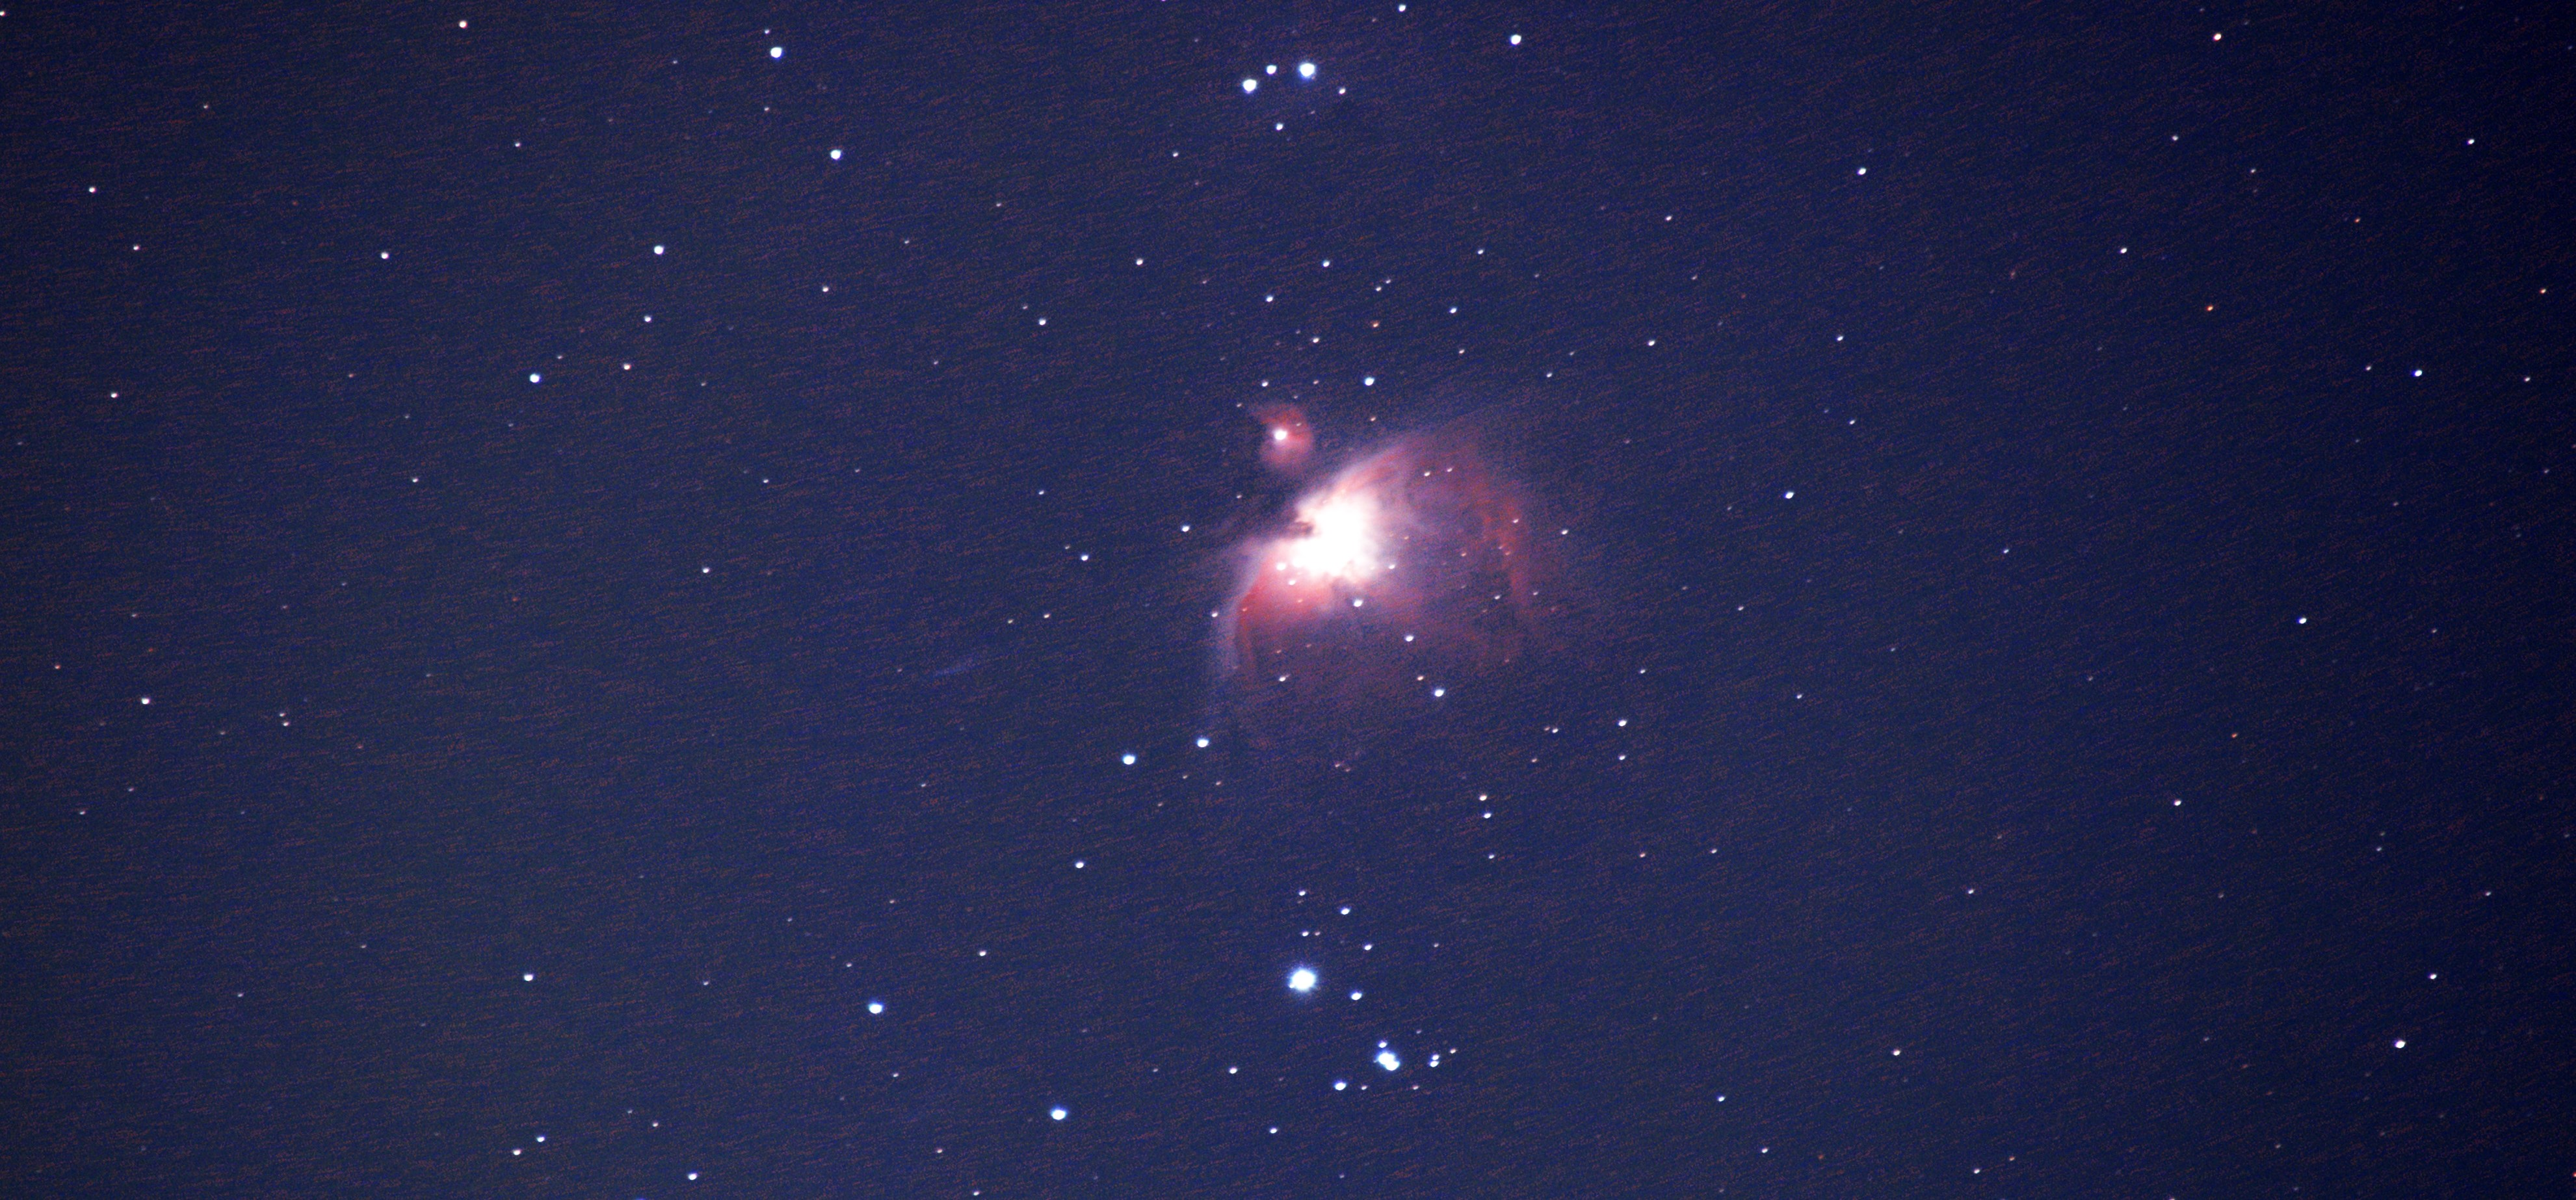
\includegraphics[width=\textwidth]{figures/Yosuke/2022_09_26_Orion_crop.jpg}
  \caption{2022年9月26日に初めて調布で撮ったオリオン大星雲(トリミング済み)\mbox{}\\EOS80D / SIGMA 18-300 F3.5-6.3 DC OS HSM / 300mm / $120\si{s} \times 5枚$(加算平均合成) / F6.3 / ISO-100 / 光害カットフィルター使用 }
  \label{fig:firstOrion}
\end{figure}
\section{都会でできる天体観測の限界に挑戦したい}
調布駅前の都市光害真っ只中で活動する電通大天文部.星なんて見えるのでしょうか.よく晴れた日にぐっと目を凝らして夜空を見つめてみると,ちらほらと星が輝いているのが見えます.肉眼で見えるような物だと,月はもちろんのこと,木星や土星などの惑星や3等星くらいまでの星が見えることになります.都会での天体観測というと大抵このあたりの星を望遠鏡で覗いてみるというのがポピュラーだと思います.私も天文部を始めた頃に望遠鏡で見た木星の縞模様の鮮明さが今でも忘れられません.
\begin{figure}[H]
  \centering
  \begin{minipage}{0.4\columnwidth}
    \centering
    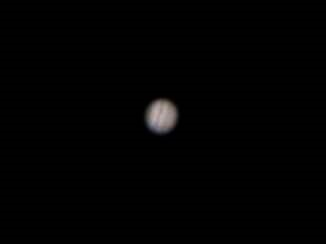
\includegraphics[width=\columnwidth]{figures/Yosuke/Jupiter.jpg}
    \caption{撮影した木星}
    \label{fig:jupiter}
  \end{minipage}
  \begin{minipage}{0.4\columnwidth}
    \centering
    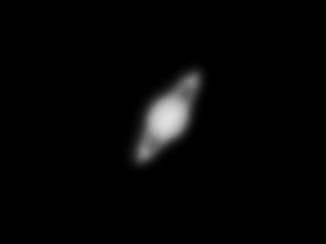
\includegraphics[width=\columnwidth]{figures/Yosuke/Saturn.jpg}
    \caption{撮影した土星}
    \label{fig:saturn}
  \end{minipage}
\end{figure}
しかし,天体観測の醍醐味と言えば淡い星雲や銀河などを見たりその姿をカメラに収めることも外せません.そういった対象を狙うには都会から離れた山奥などの暗い場所まで大きい天体望遠鏡を運んで夜通し露光したりすることが一般的です.これができるに越したことはありませんが,私たちは大学生です.学業が本分である以上,そう頻繁に遠くへ出かけることもできないし,お金もない.夜通し観測していては次の日の授業を寝過ごしてしまいます.淡い星雲や銀河をこの目で見て撮りたい欲求と学生の本分は全うしたい,この相反する2つの項をなんとかクリアするため,この明るい東京の空で星雲や銀河の観測に挑戦しています.

一見無謀にも思えますが,カメラで長時間露光をすると肉眼よりも多くの星が確認できます.つまり,肉眼ではっきりと見ることは叶わなくとも,カメラで撮影することはできる訳です.さらに,条件が良ければ東京の空からでも肉眼で見ることができる明るくて大きな星雲が存在します.そう,オリオン大星雲です.
\section{オリオン大星雲とは}
オリオン大星雲はオリオン座のオリオンの股下に当たる部分にある散光星雲です.秋から冬にかけて見ることができます.メシエカタログの42番目として「M42」の名で呼ばれることもあります.

鳥が翼を広げたような形が特徴的で,星雲の中央部にはトラペジウムと呼ばれる明るい4つの星が集まっています.トラペジウムは太陽の数十倍,約4万度の高温に達することで強烈な紫外線を放ち,周囲のガスやチリをも輝かせています.

オリオン座自体が明るい星(0等星2つ,2等星5つ)で構成されていて,その形も特徴的であることから市街地でも簡単に見つけることができます.オリオンのベルト状に並んだ2等星の三ツ星の下側に縦に並んだ「小三ツ星」というのが見られます.そのうちの中央の1つがオリオン大星雲で,双眼鏡でもうっすらとその形を見ることができます.そうしたことから,天文初心者の練習台などによく用いられる天体の1つとなっていたりします.
\begin{figure}
  \centering
  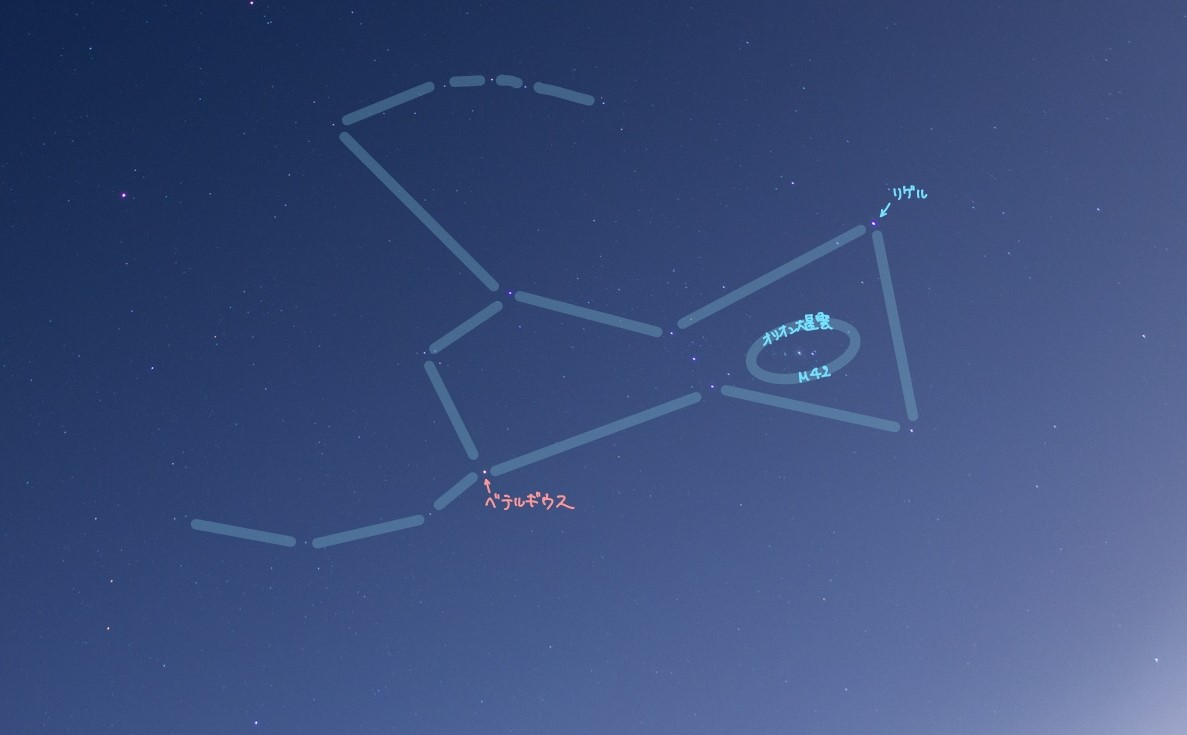
\includegraphics[width=10cm]{figures/Yosuke/Orion_line-2.jpg}
  \caption{オリオン座とオリオン大星雲の位置関係}
  \label{fig:Orion}
\end{figure}
\section{実際に撮ったオリオン大星雲}
冒頭の\figref{firstOrion}は,調布市総合体育館屋上で,9月26日に自分の手持ちの機材で撮ったオリオン大星雲です.赤道儀で追尾しながらではありますが,普通のカメラレンズで撮った物になります.光害カットフィルターという星雲が主に放つ光の波長帯を通し,それ以外の都市の光に多い波長帯を遮断するものを使ったため,星雲自体の姿をしっかりと映し出せていると思います.

\subsection{調布と福島での比較}
夏合宿で行った福島県裏磐梯で撮影したオリオン大星雲(\figref{FukushimaOrion})とその後に調布市総合体育館屋上で撮影したオリオン大星雲(\figref{ChofuOrion})を比較してみます.機材はどちらも天文部のFC-76というフローライトの屈折望遠鏡と私のEOS80Dという一眼レフを用いています.この望遠鏡用の光害カットフィルターは準備できなかったので,光害の有無がはっきりと出ます.やはり福島で撮影した物の方(\figref{FukushimaOrion})に分があります.多少ノイズが気になりますが,この写真は10秒1枚撮りです.色調整以外はほとんど撮って出しに近い状態です.ここ重要なので覚えておいてください.調布で撮った方(\figref{ChofuOrion})も,一見すると同じくらいの写りになっているかと思います.しかし,こちらは1秒露光180枚を30枚ずつ加算した6セットを加算平均した\footnote{実質の露光時間は30秒ということになるでしょうか.}後にPhotoshopで無理矢理明るさを持ち上げて星雲を浮かび上がらせている代物です.そのため画像には縦線のようなノイズが発生してるようにも見えます.
\begin{figure}[H]
  \centering
  \begin{minipage}{0.4\columnwidth}
    \centering
    \vspace{3.7mm}
    \includegraphics[width=\columnwidth]{figures/Yosuke/Astro-Kuore082.JPG}
    \vspace{-1.5\zw}
    \caption{福島県裏磐梯のオリオン大星雲}
    \label{fig:FukushimaOrion}
  \end{minipage}
  \begin{minipage}{0.4\columnwidth}
    \centering
    \includegraphics[height=\columnwidth, angle=-90]{figures/Yosuke/Orion_221019.jpg}
    \caption{調布のオリオン大星雲}
    \label{fig:ChofuOrion}
  \end{minipage}
\end{figure}

調布で撮影した方は1秒露光を181枚撮ったので,全部加算して181秒露光相当にすることもできます.参考までに加算後の画像と強調処理後の画像を載せておきます.加算直後の画像がほぼ真っ暗で,中央に薄ぼんやりとしたものが見えるかと思います.見えているのはトラペジウムくらいで,翼を広げた鳥のような雲の形はわかりません.明るさなど調整して強調処理すると,雲のディティールなどがわかるようになります.181秒相当なだけあって,細部のディティールも描き出すことができますが,それだけ周辺部分も明るいので,コントラストが低くなってしまいます.
\begin{figure}[H]
  \centering
  \begin{minipage}{0.4\columnwidth}
    \centering
    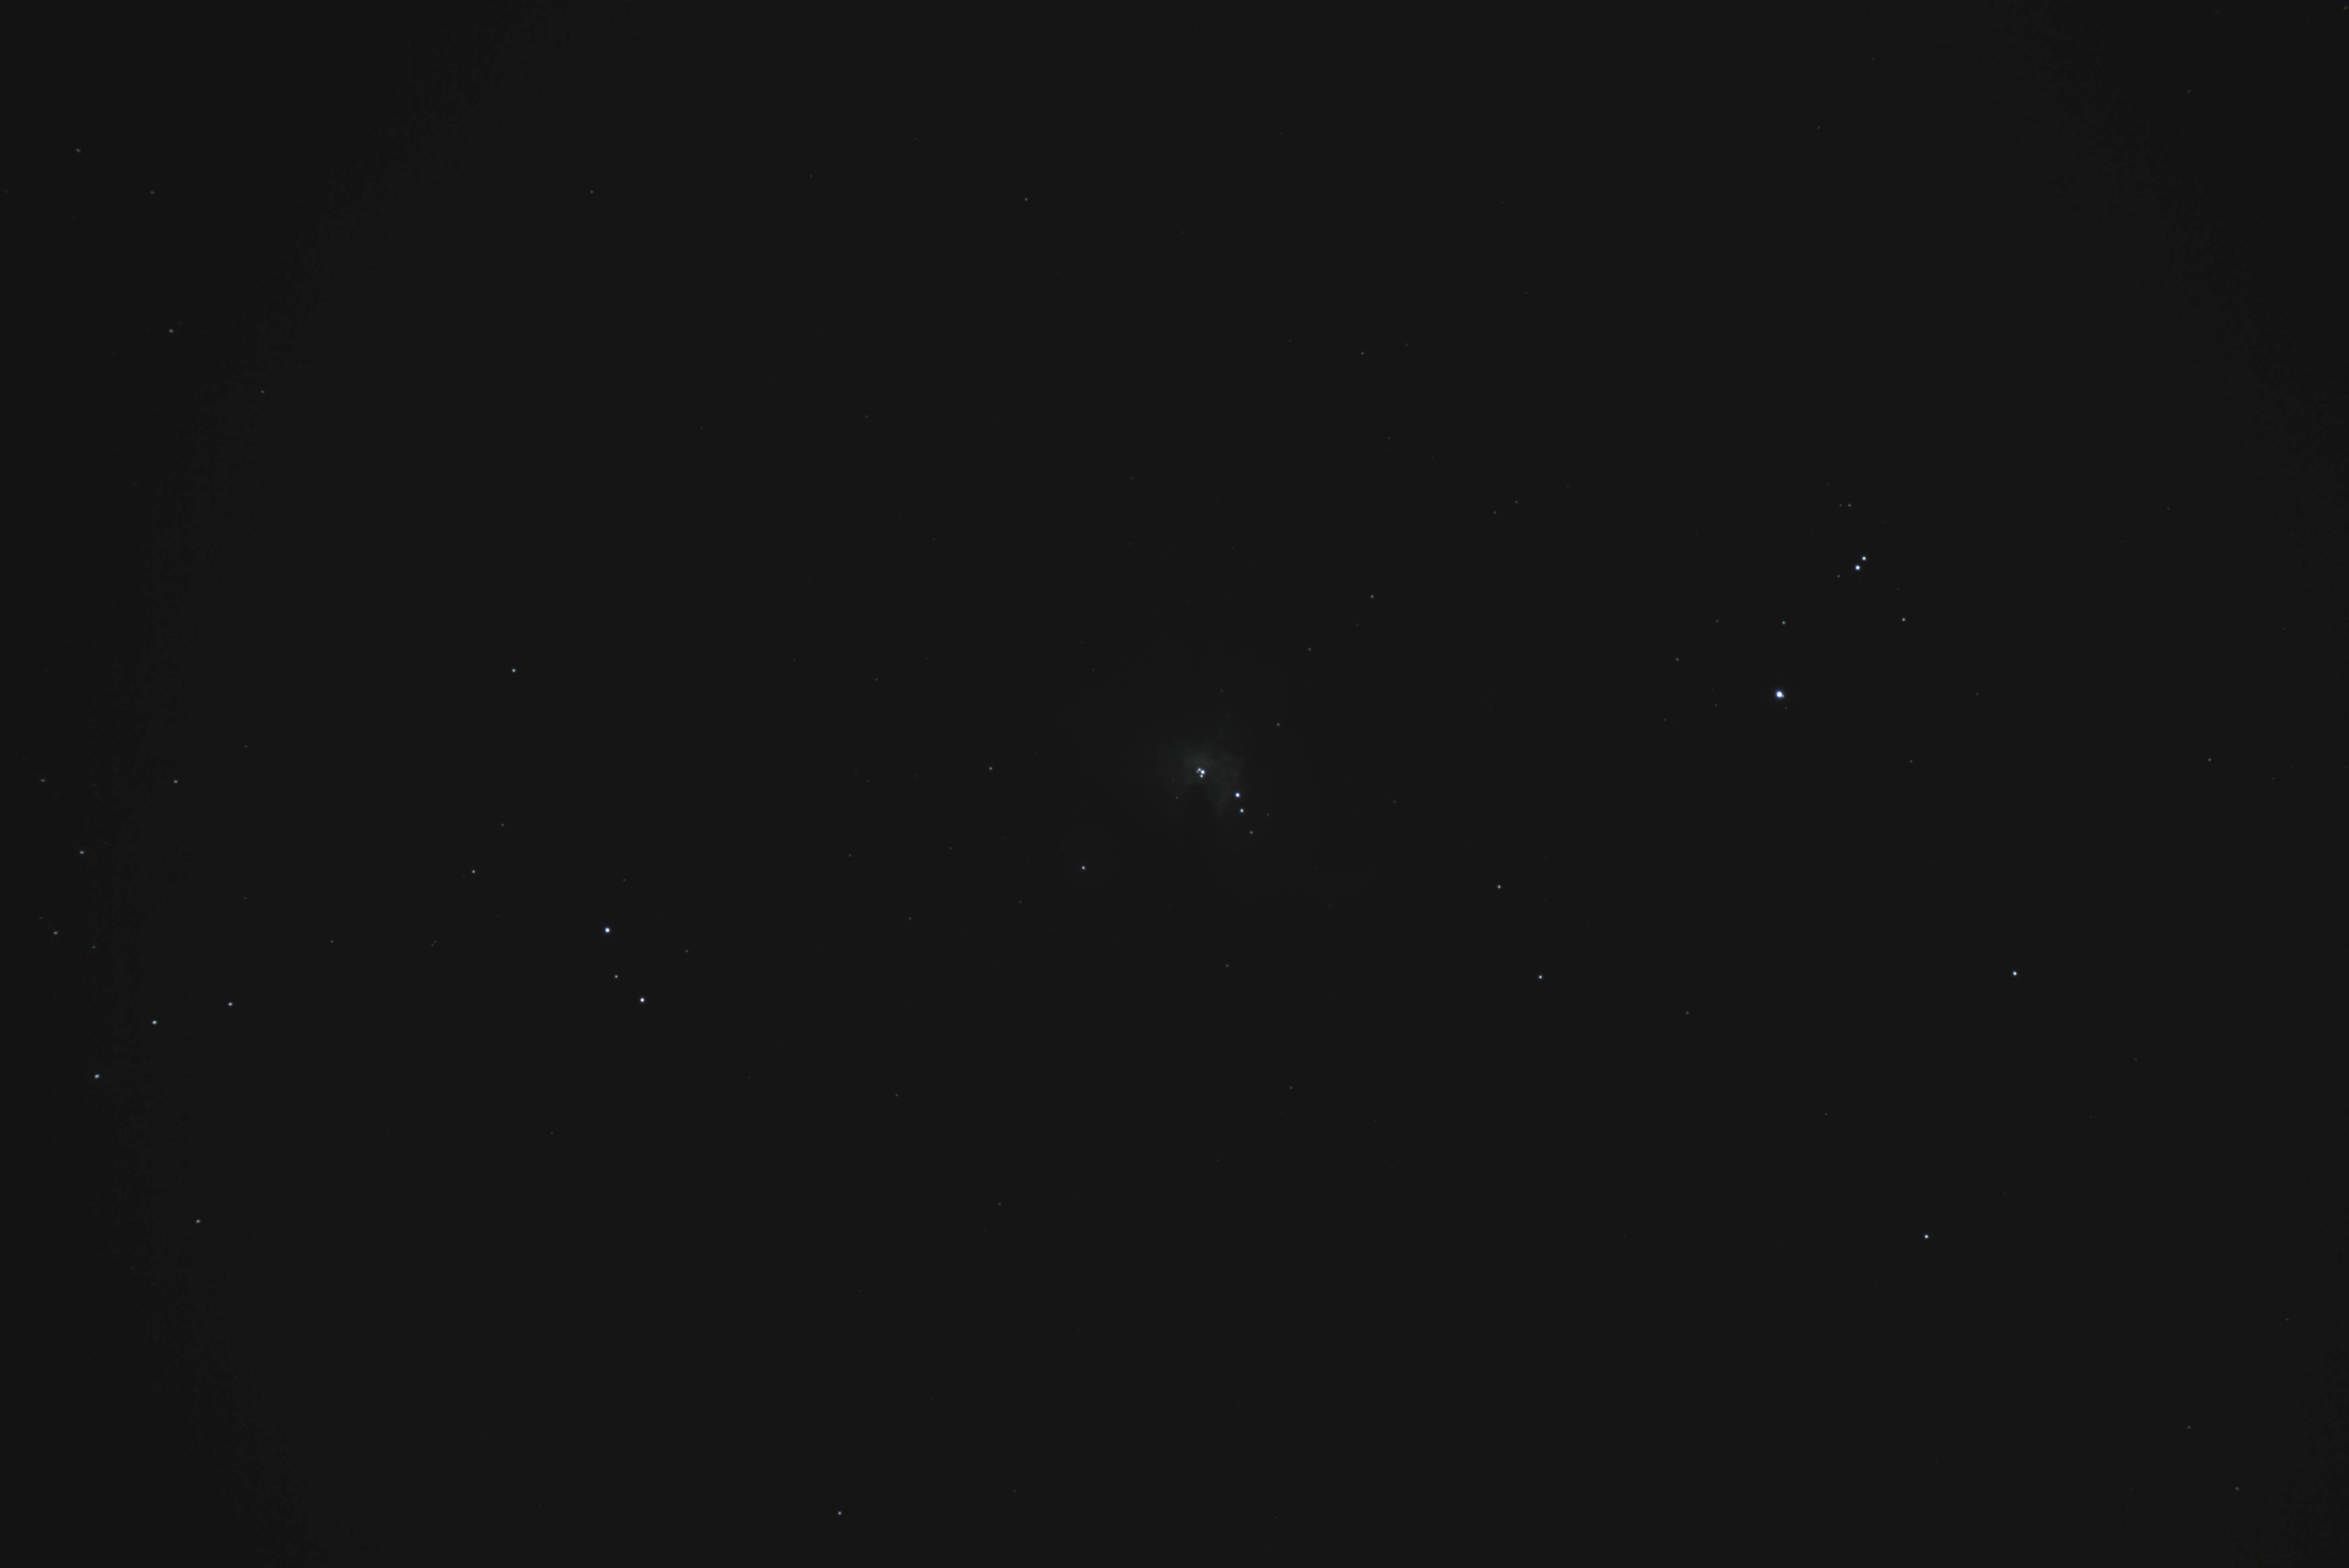
\includegraphics[width=\columnwidth]{figures/Yosuke/Orion_181coposit_non.jpg}
    \caption{加算直後の181枚加算画像}
    \label{fig:Orion_181coposit_non}
  \end{minipage}
  \begin{minipage}{0.4\columnwidth}
    \centering
    \includegraphics[width=\columnwidth]{figures/Yosuke/Orion_181coposit.jpg}
    \caption{強調処理後の181枚加算画像}
    \label{fig:Orion_181coposit}
  \end{minipage}
\end{figure}

\section{場所は調布駅前電通大!向かうは天文部の巨砲NGT-18!}
これまで,調布でとはいっても比較的暗い調布市総合体育館屋上で撮影したオリオン大星雲を見てきました.合宿にしろ調布市総合体育館屋上での観測にしろ,移動を伴うためあまり大きい天体望遠鏡を運ぶことができません.淡い光を捉えるためには集光力が重要となるので,口径の大きな望遠鏡で撮ってみたくなります.

我が電通大天文部には,NGT-18という口径45cmの巨砲が存在しています.技術的には持ち運びが可能ですが現実的ではなく,専ら活動拠点である東3号館屋上の天体観測ドームに鎮座しています.電通大の立地上,調布駅のすぐ近くという光害の最も激しい地域に望遠鏡が置かれているため,その集光力は余り発揮せずに月や惑星を狙うことがほとんどでした.
\begin{figure}[H]
  \centering
  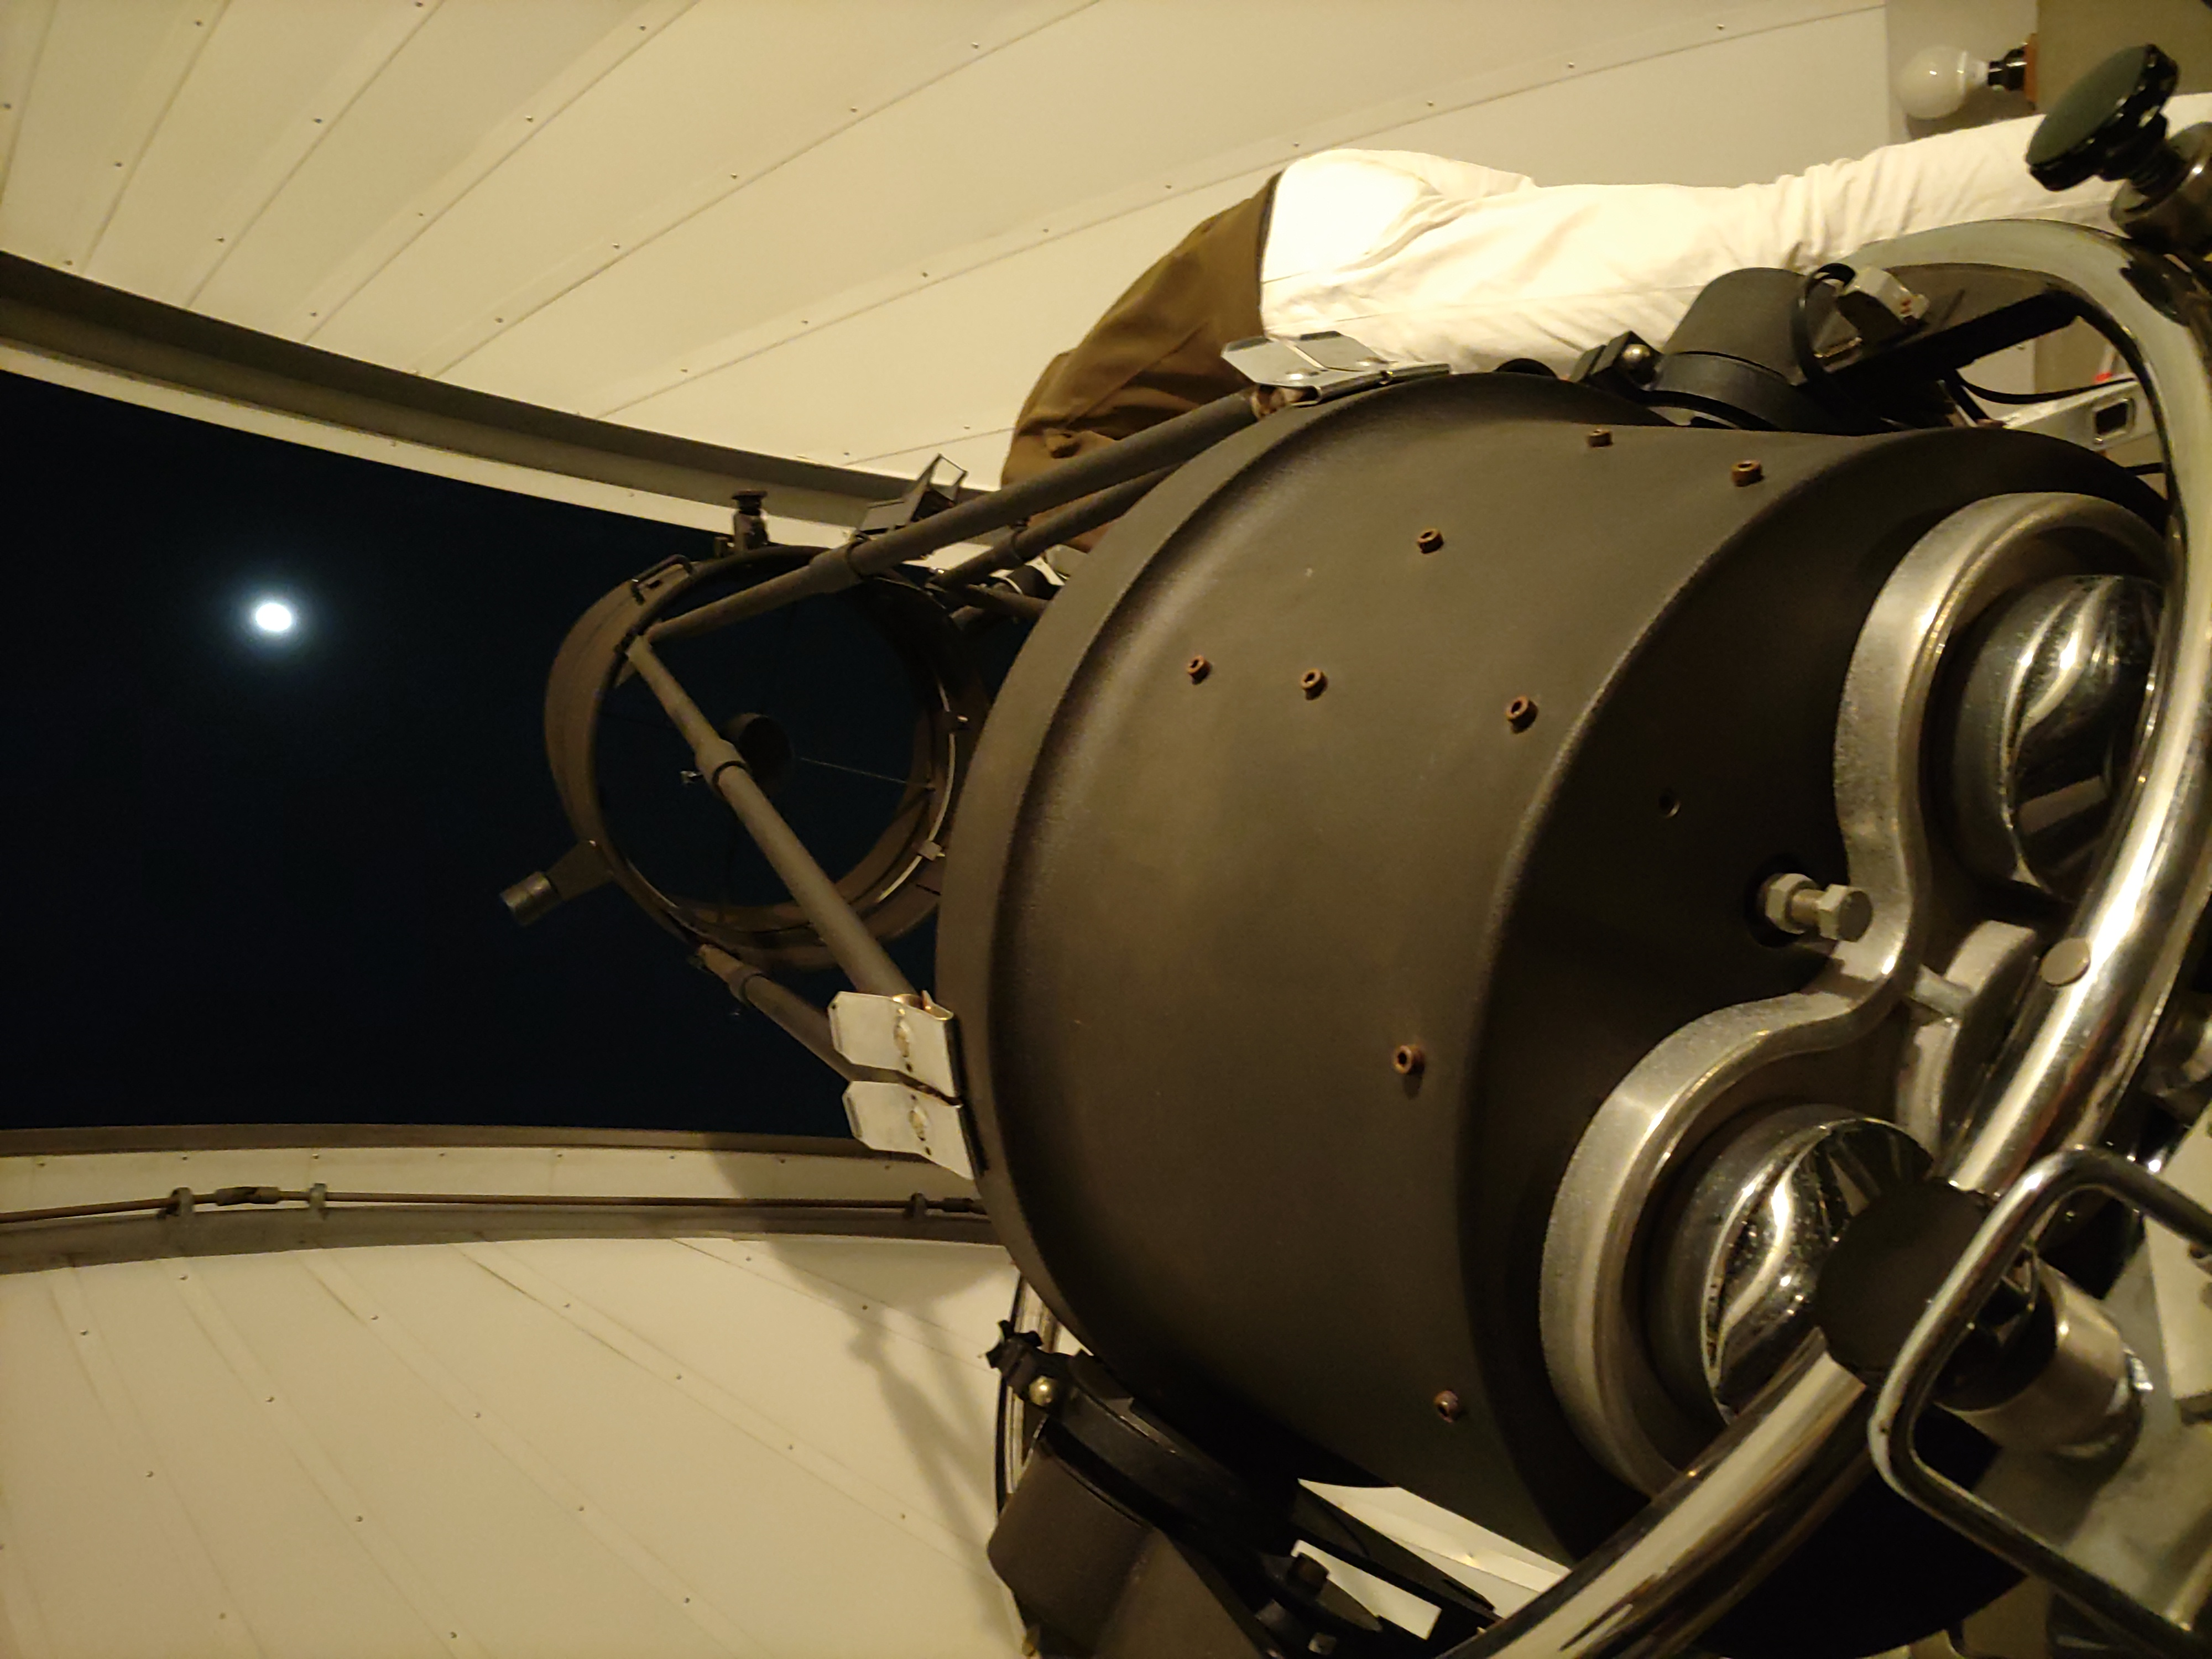
\includegraphics[height=8cm, angle=-90]{figures/Yosuke/NGT-18.jpg}
  \caption{電通大天文部の巨砲 NGT-18}
  \label{fig:NGT-18}
\end{figure}
なんとかしてこの集光力を活かしてオリオン大星雲を撮ってみたい.そのためにNGT-18に取り付けられる光害カットフィルターやカメラを取り付けるためのアダプターなども準備しました.役者はそろいました.ファインダーが使えない状態でも当時の部長がオリオン大星雲を導入してくれました.うっかりカメラは20年前のEOS 10Dですが,理論上は写りに問題ないはずです.さて,調布駅前の都市光害vs電通大天文部の巨砲はどちらが勝つのでしょうか.
\begin{figure}[H]
  \centering
  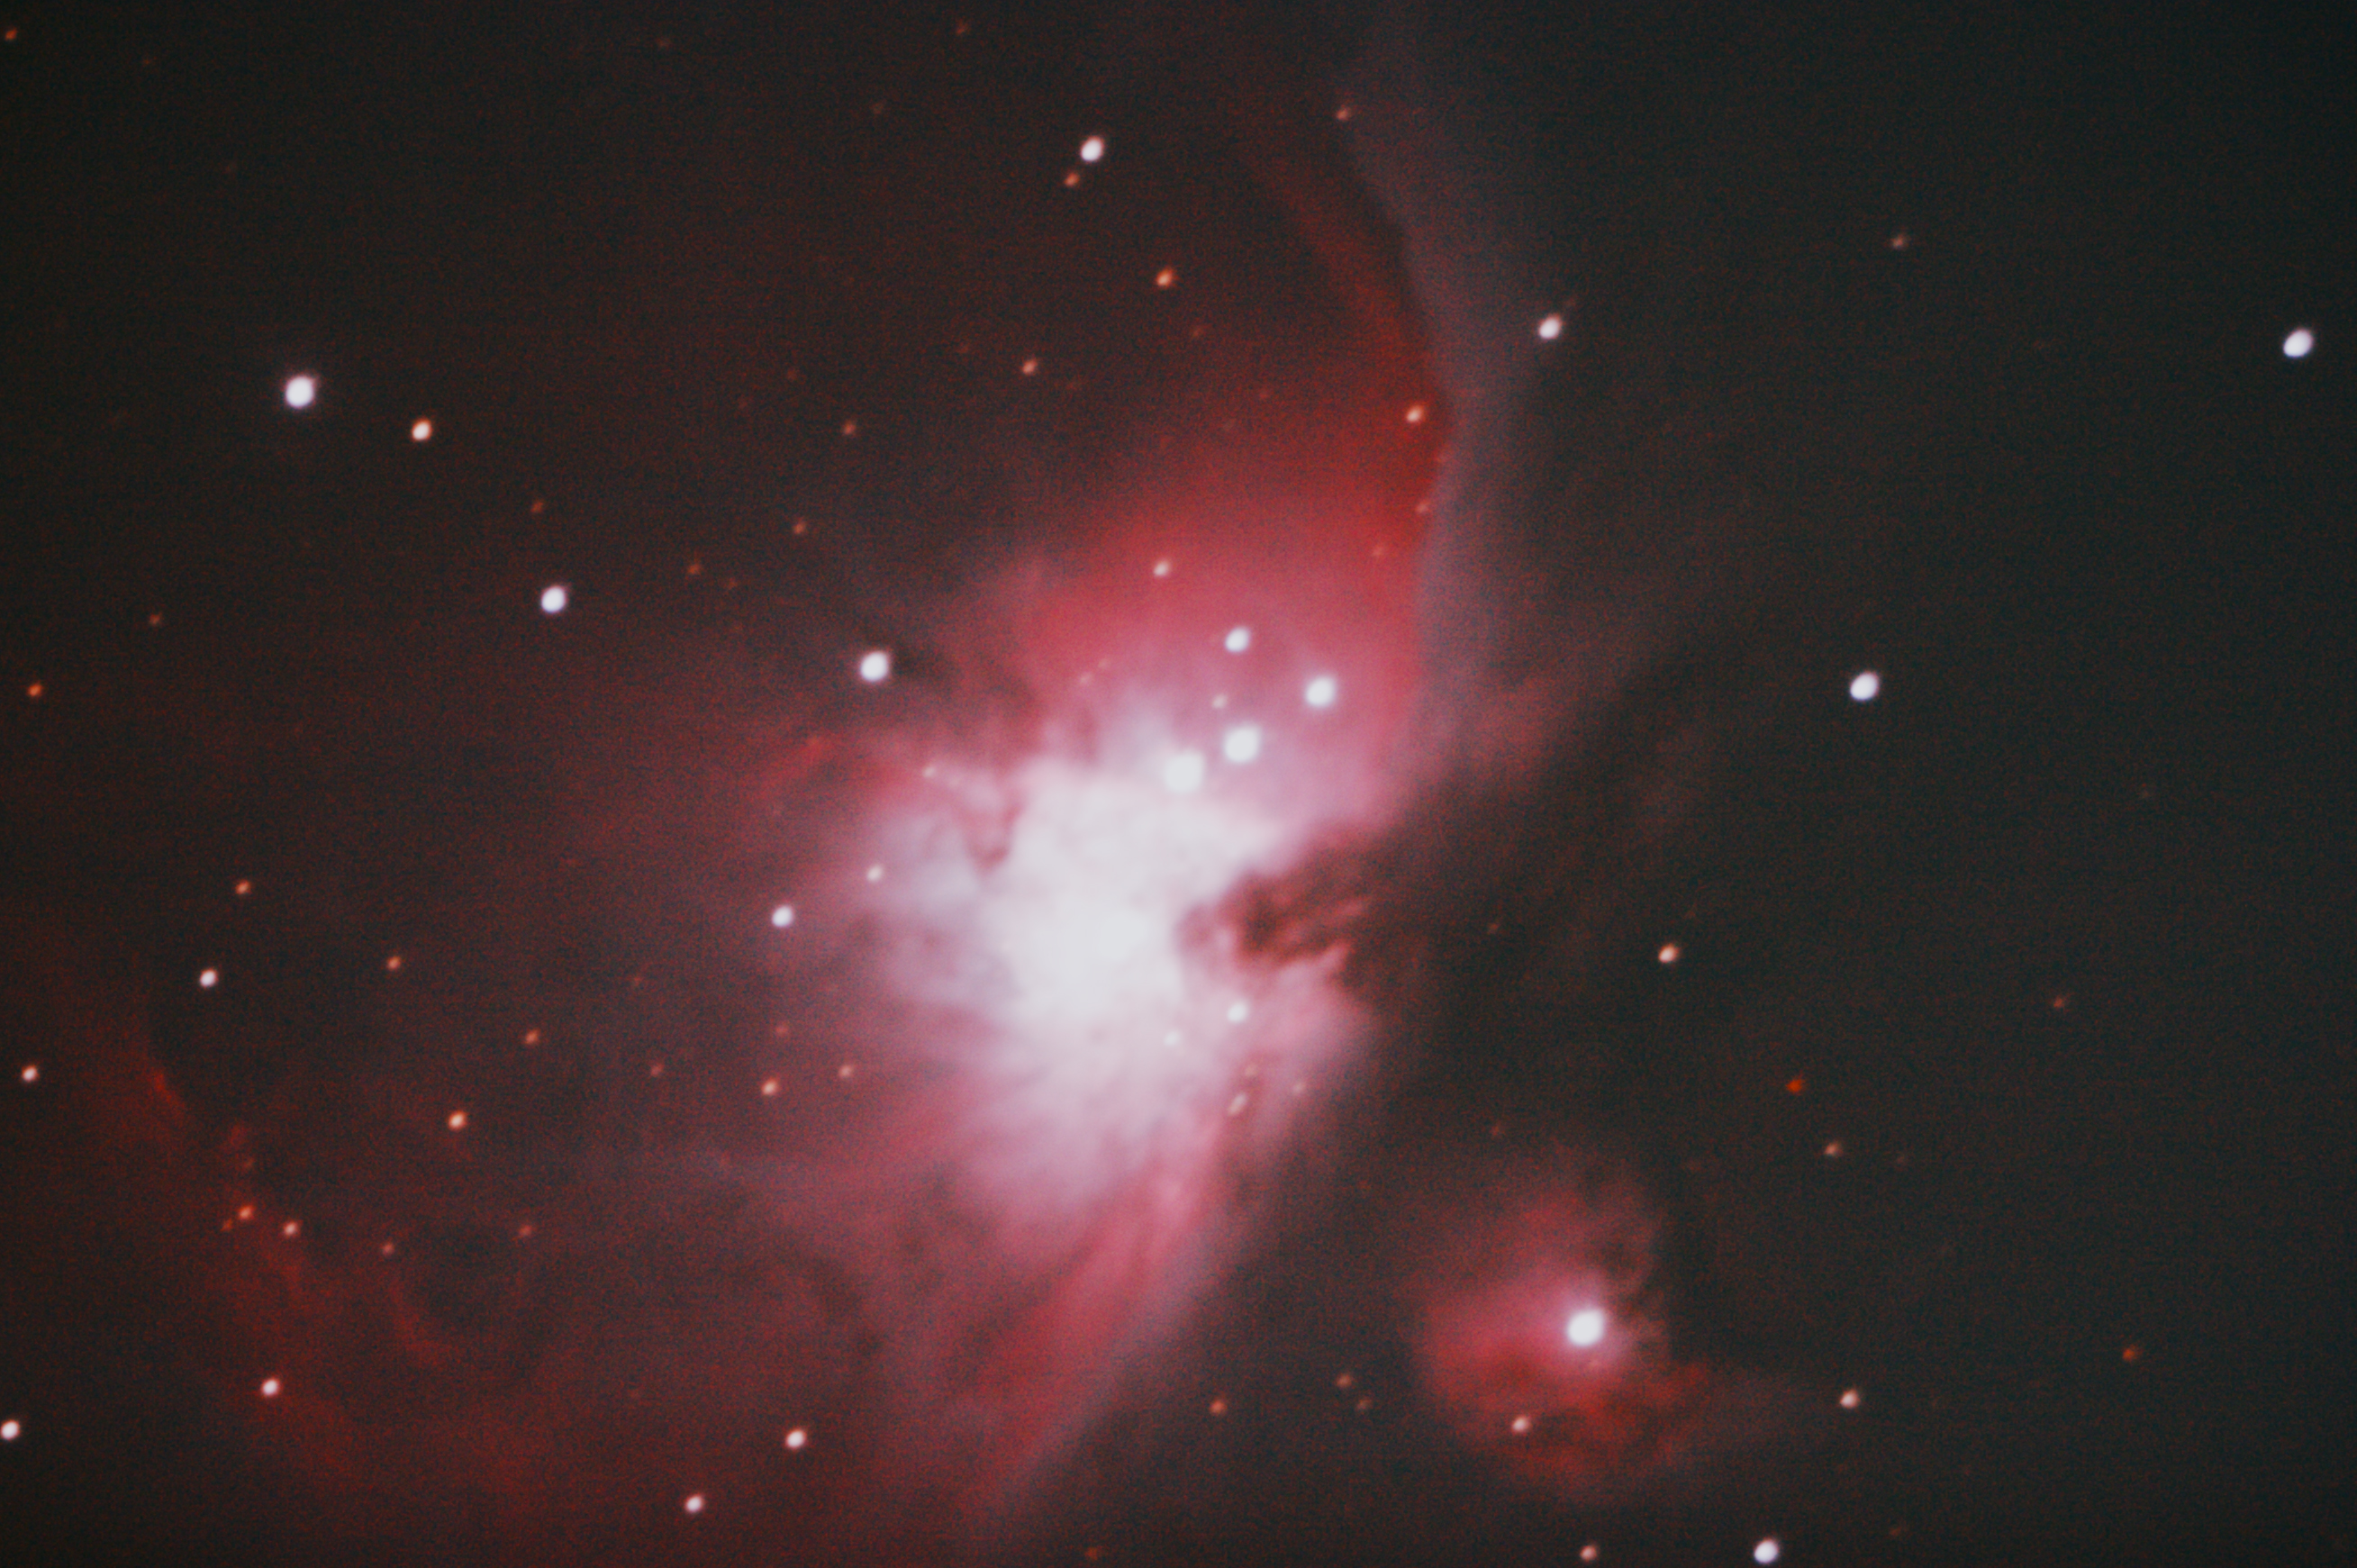
\includegraphics[width=.8\textwidth, angle=180]{figures/Yosuke/2023_01_10_Orion_Chofu_NGT-18_5-Composit.jpg}
  \caption{NGT-18とEOS10Dで撮ったオリオン大星雲}
  \label{fig:NGTOrion}
\end{figure}
すこし眠い写りですが,かなりいい具合に撮れてるのではないでしょうか.眠くなってる原因としては巨体によるブレや鏡面の光軸のずれ,カメラの画素数が少ないことが考えられると思います.次の2枚は撮って出しでの光害カットフィルターありとなしの比較です.紙面ではすこしわかりづらい気もしますが,こうしてみると光害カットフィルターによってコントラストが向上していることがわかります.
\begin{figure}[H]
  \centering
  \begin{minipage}{0.3\columnwidth}
    \centering
    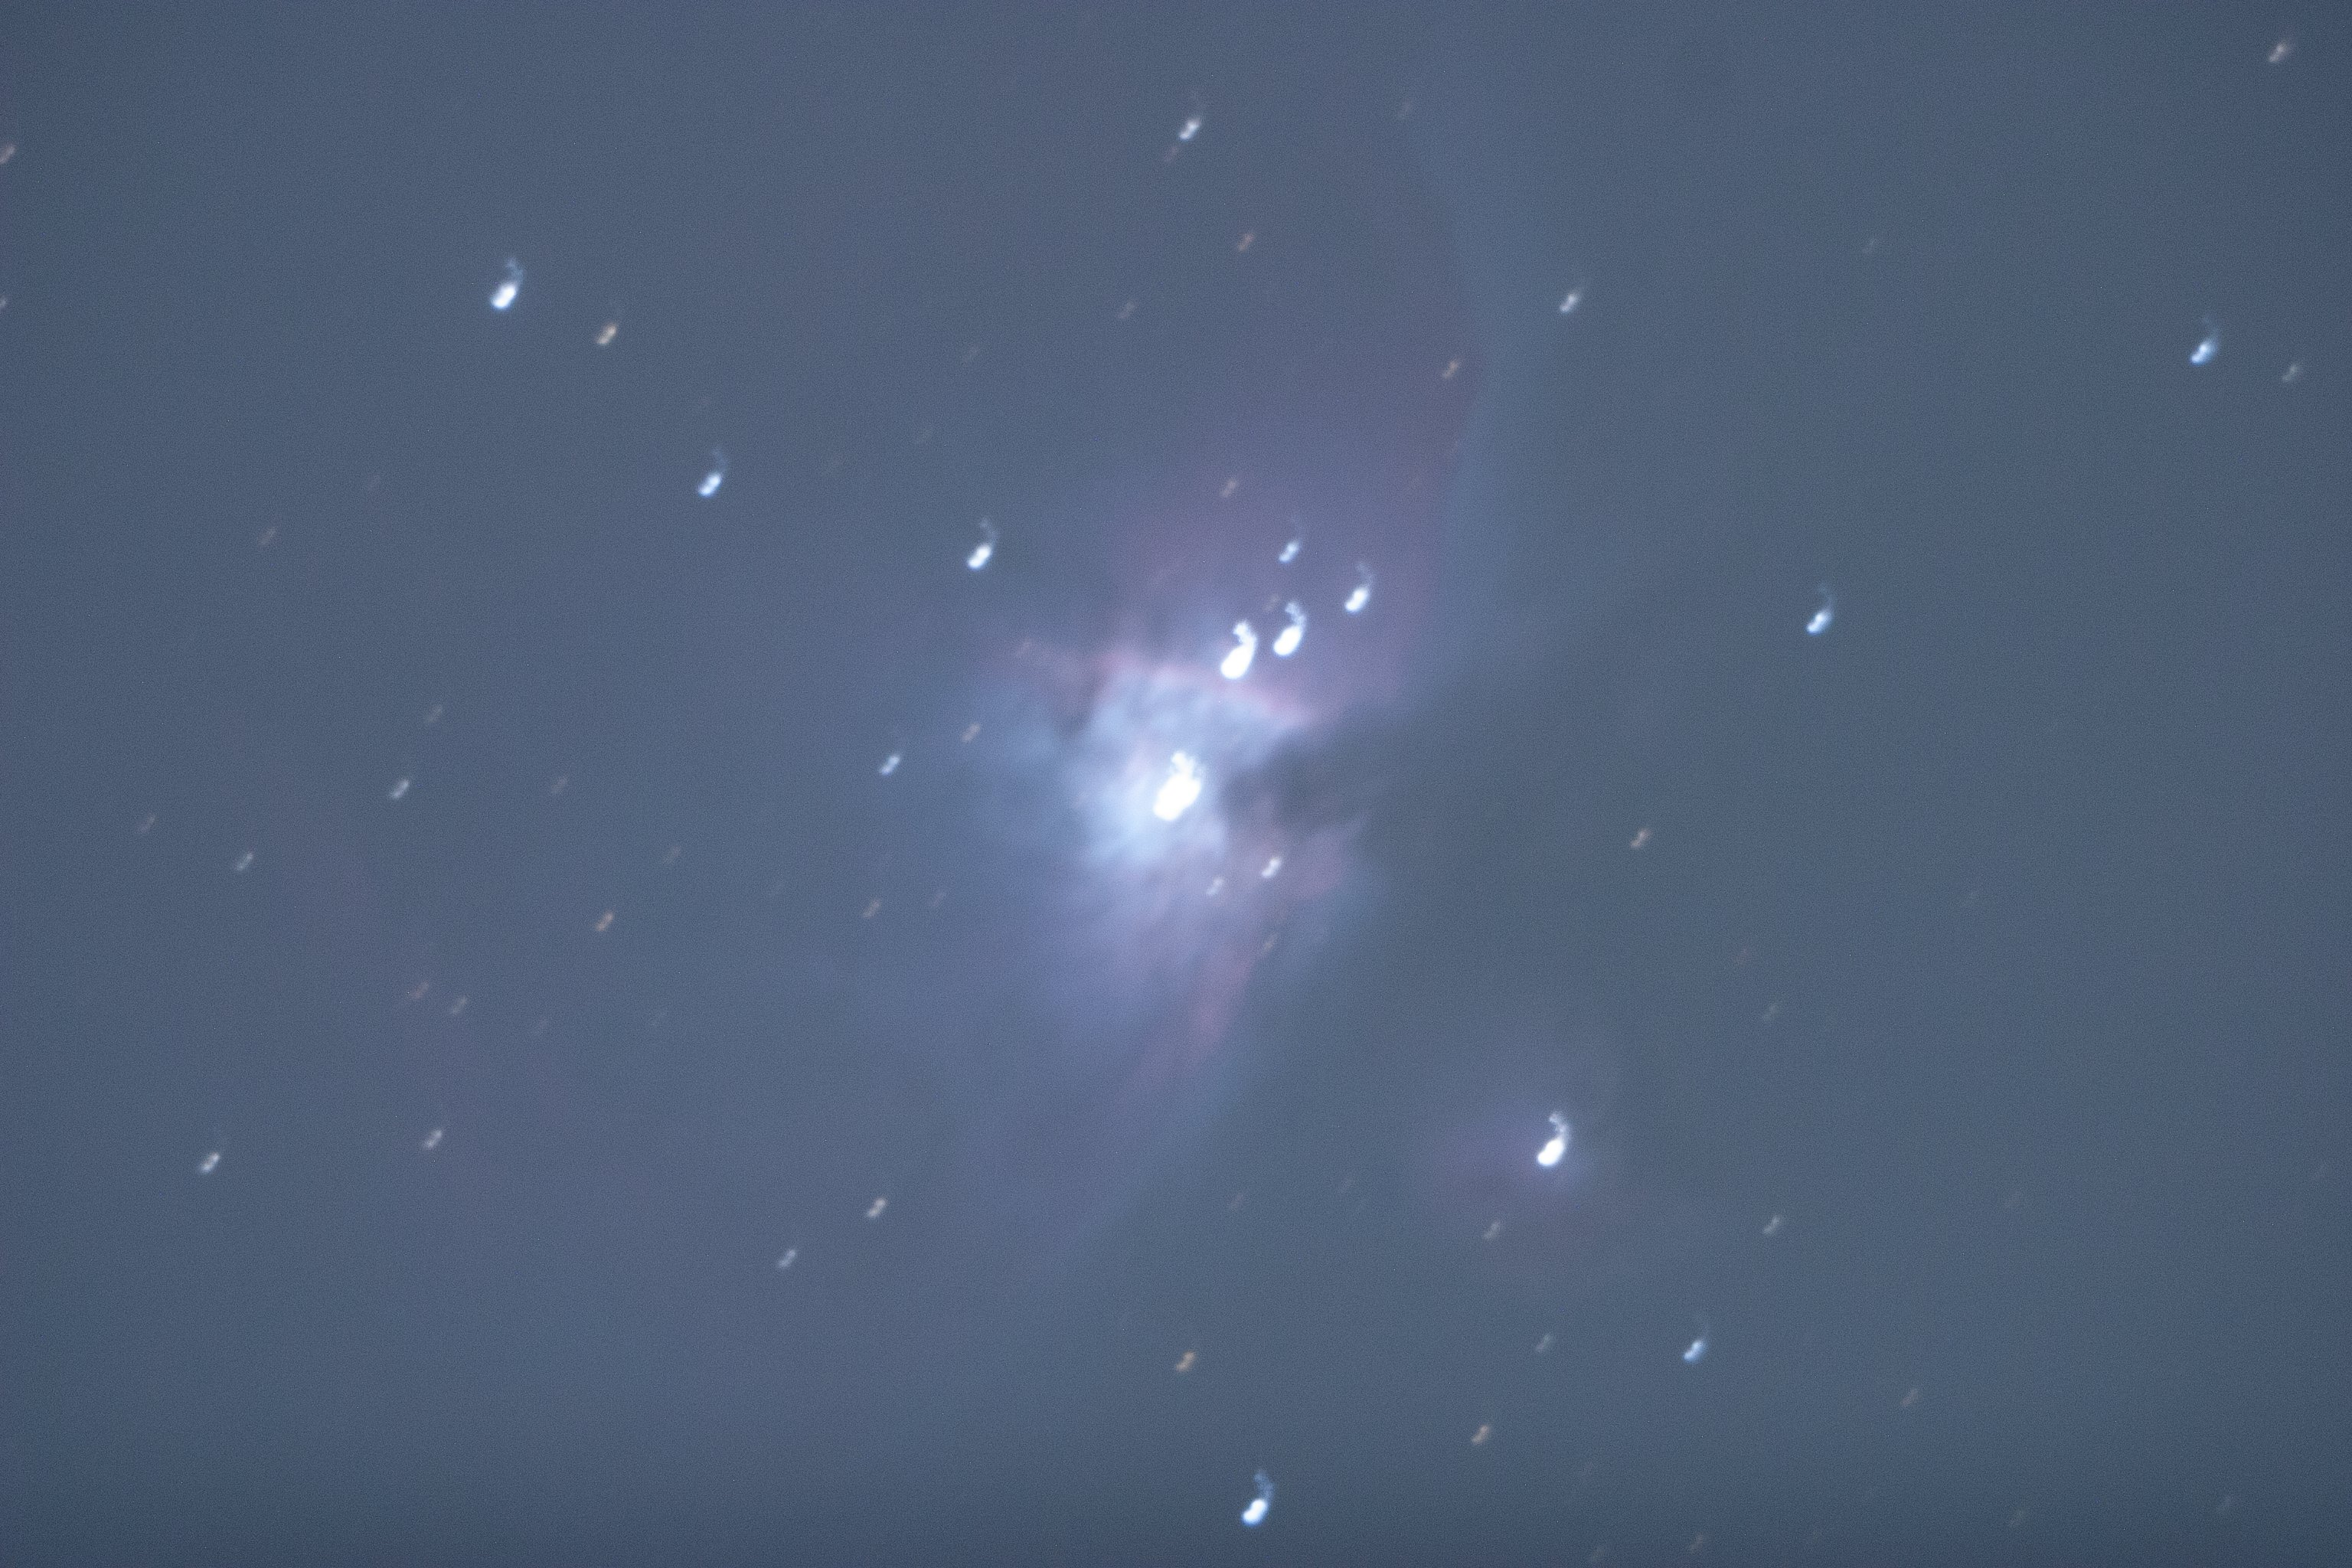
\includegraphics[width=\columnwidth, angle=180]{figures/Yosuke/orion_ngt18_non.jpg}
    \caption{光害カットフィルターなし}
    \label{fig:orion_ngt18_no}
  \end{minipage}
  \begin{minipage}{0.3\columnwidth}
    \centering
    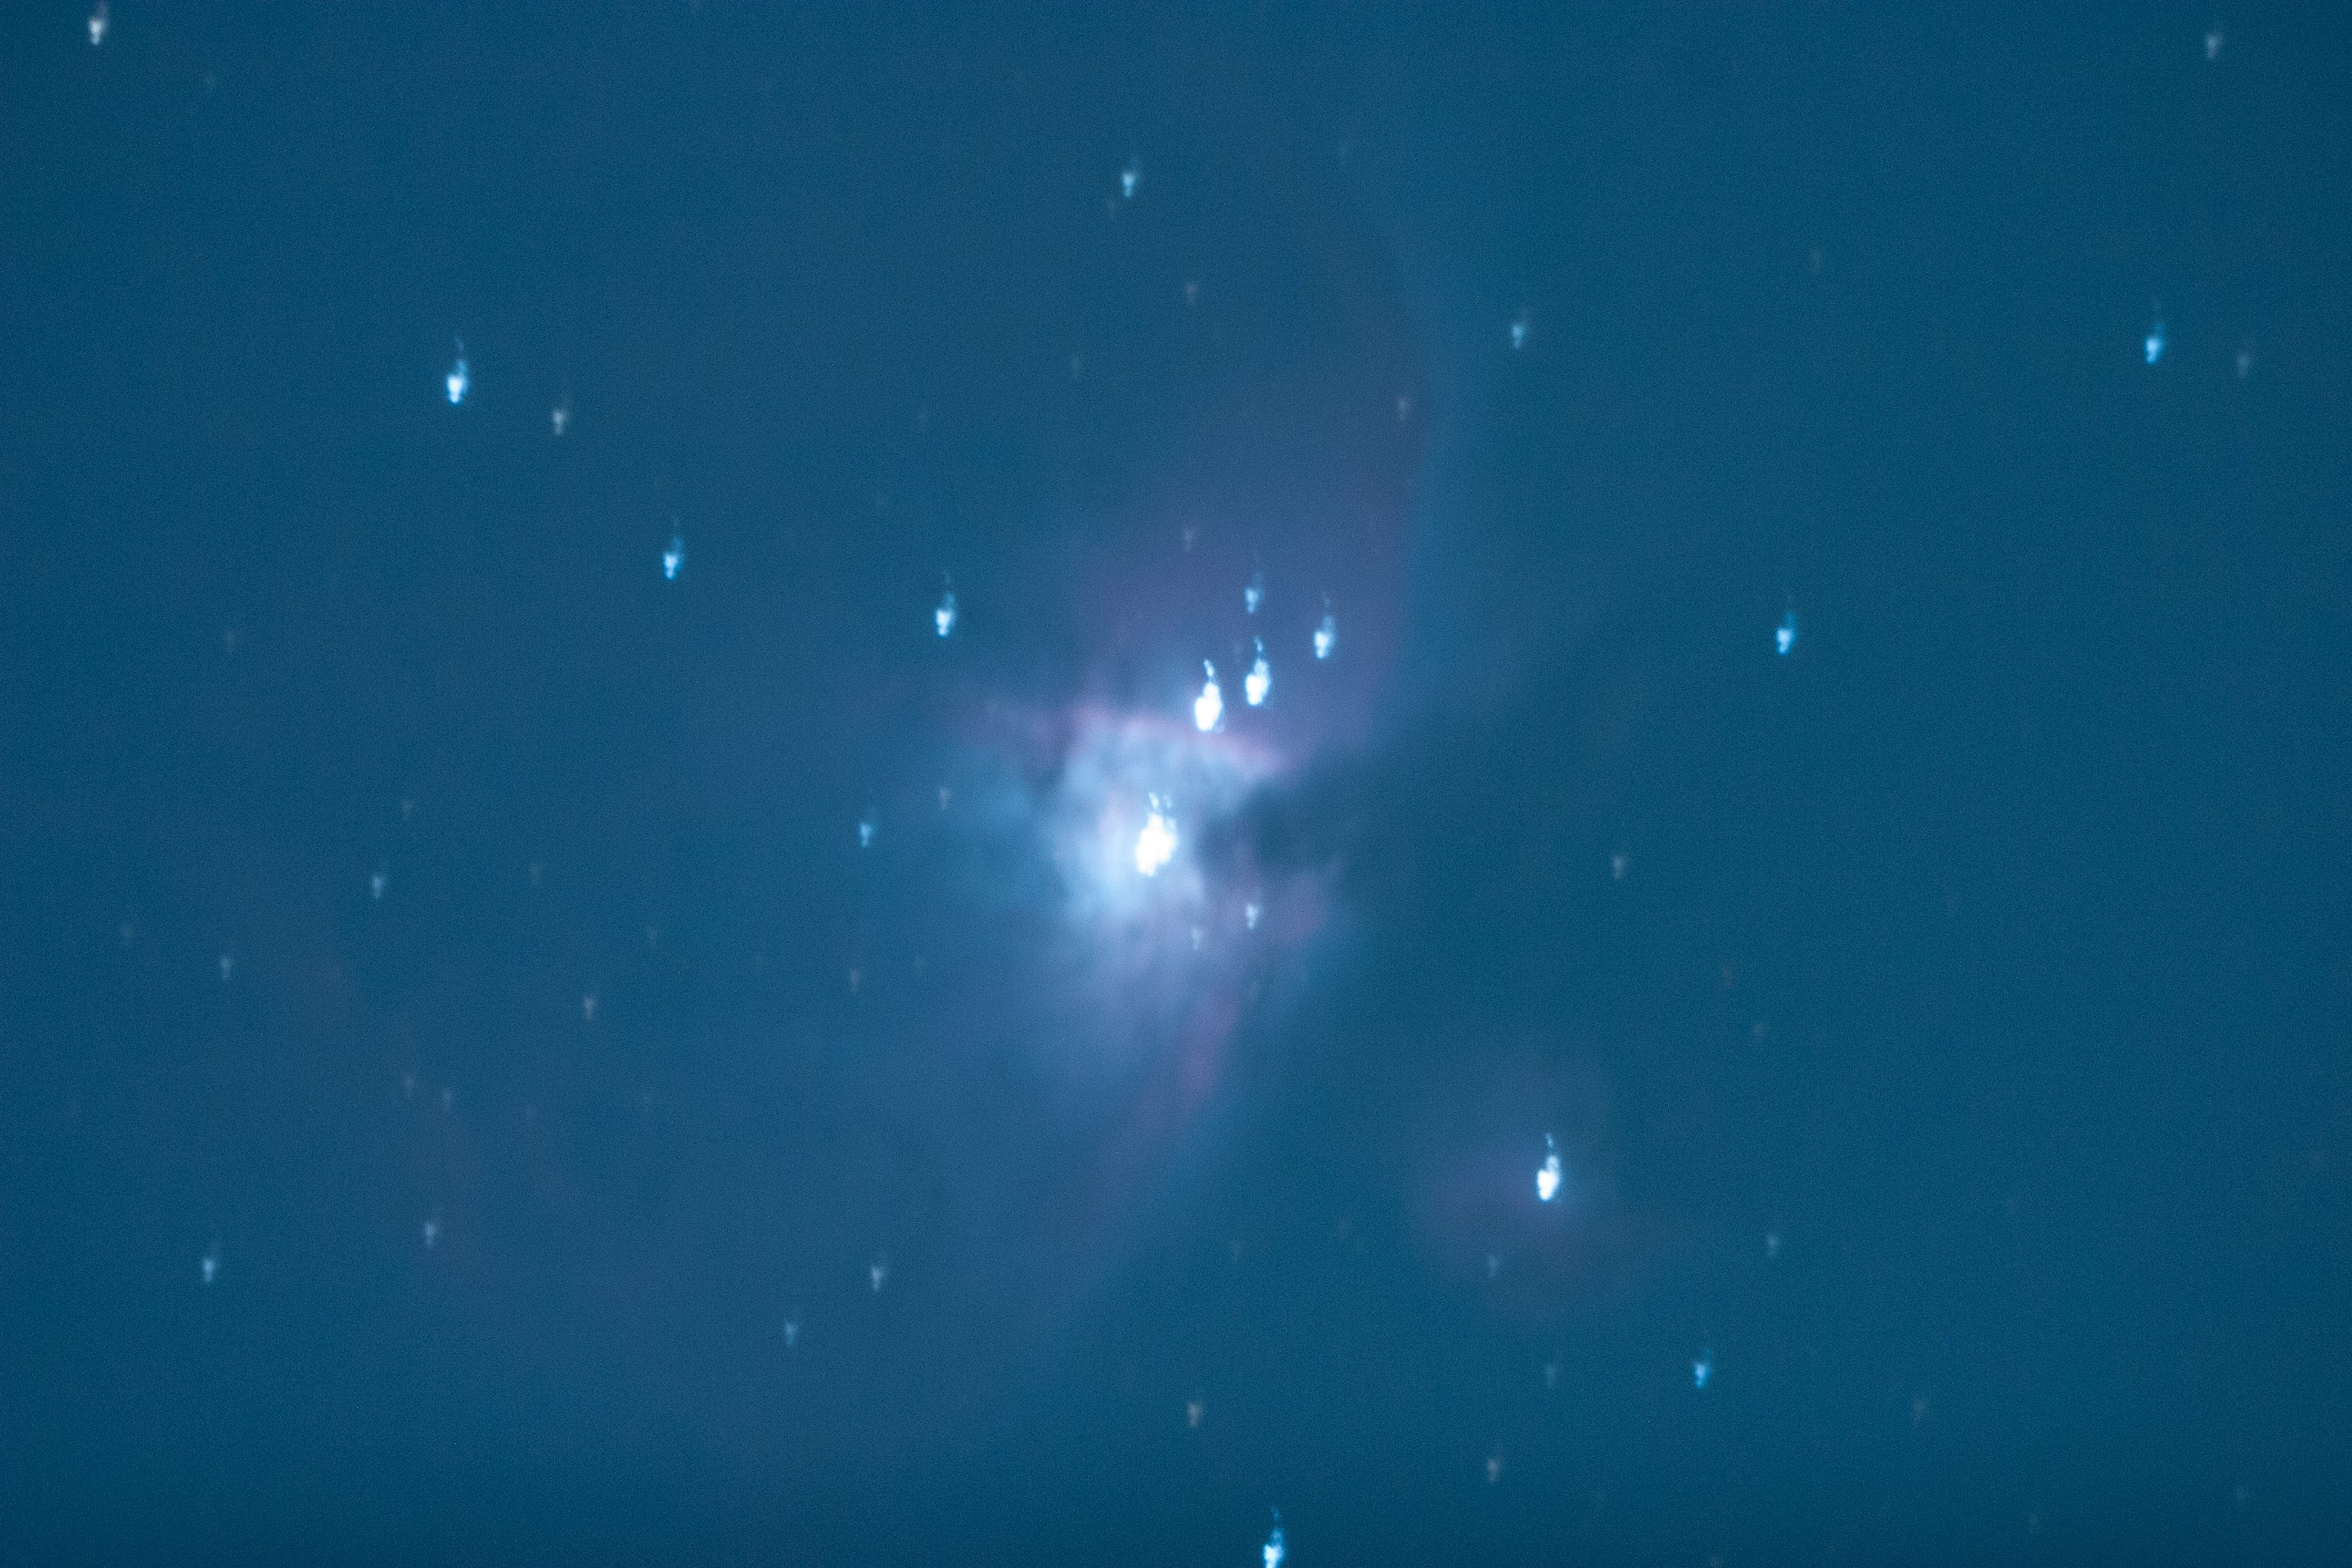
\includegraphics[width=\columnwidth, angle=180]{figures/Yosuke/orion_ngt18_cut.jpg}
    \caption{光害カットフィルターあり}
    \label{fig:orion_ngt18_cut}
  \end{minipage}
\end{figure}

\section{さいごに}
今回は調布でオリオン大星雲を撮影したことについて書いてきました.特に巨砲NGT-18でオリオン大星雲を撮影するのは私が天文部でやり遂げたかったことの一つだったので,達成できてとてもうれしいです.まだまだ写りの改善点や画像処理の分野などで取り組むべき点も多いですが,ひとまず調布のような明るい空からでも,淡い天体を撮影することができるということがみなさんにお伝えできれば幸いです.今後はもっと淡い天体などいろいろな種類の天体を撮影して,天体写真のブースをもっと彩りよく飾れればと思います.
\begin{thebibliography}{1}
  \bibitem{messier} 中西昭雄,メシエ天体&NGC天体ビジュアルガイド,誠文堂新光社,2017年,p.92
  \bibitem{orion} 星から宇宙へ,オリオン大星雲とトラペジウム,\url{https://www.city.ibara.okayama.jp/hosikarautyuuhe/R2/r3.2.html}, 2023/03/06
\end{thebibliography}
% https://www.city.ibara.okayama.jp/hosikarautyuuhe/R2/r3.2.html
\end{document}
